\documentclass{article}
\usepackage{graphicx} % new way of doing eps files
\usepackage{listings} % nice code layout
\usepackage[usenames]{color} % color
\definecolor{listinggray}{gray}{0.9}
\definecolor{graphgray}{gray}{0.7}
\definecolor{ans}{rgb}{1,0,0}
\definecolor{blue}{rgb}{0,0,1}
% \Verilog{title}{label}{file}
\newcommand{\Verilog}[3]{
  \lstset{language=Verilog}
  \lstset{backgroundcolor=\color{listinggray},rulecolor=\color{blue}}
  \lstset{linewidth=\textwidth}
  \lstset{commentstyle=\textit, stringstyle=\upshape,showspaces=false}
  \lstset{frame=tb}
  \lstinputlisting[caption={#1},label={#2}]{#3}
}


\author{Shaun Gordon and Sam Sahli}
\title{Lab 1 - Introduction}

\begin{document}
\maketitle

\section{Introduction}
The purpose of this lab was to test a 32 bit register and guarantee it was operating correctly. The test bench was designed to test every bit in the register as well as the clock and the reset. If the lab was executed correctly, the test bench will have proven the operation of the 32 bit register with minimal test inputs.

\section{Interface}
The 32 bit register tested in this lab consisted of a clock input, a reset input, a 32 bit register input, and a 32 bit wire output. These inputs and outputs were manipulated and tested with a Verilog test bench. The clock was run with a separate module titled oscillator. In order to operate correctly the clock had to be connected to the oscillator module and initialized in the test bench. The reset was controlled in the test bench. The values assigned to the 32 bit register input, D, were assigned in the test bench. The transfer from the D register to the Q output is controlled in the register module. 

\section{Design}
In order to operate correctly the 32 bit wire output, Q, would copy the data on the 32 bit register input, D, on the positive edge of every clock cycle. Subsequently, the D register would be set to zero on the positive edge of every reset pulse. This reset would also cause the Q output to be zero. The D register would also have to hold the value assigned to it until reassigned or reset. It should be built so the data is on the D register longer than a single clock cycle, or it will not be copied to the Q output. 

\section{Implementation}
All of the register module code is displayed in Listing~ \ref{code:reg} on page~ \pageref{code:reg}. The first line in the Verilog code includes a header file, definitions.vh, that contains variables used in this register module. The purpose of this header file is to allow global changes in bit width to be made without having to change each individual assignment. Next, the clock, reset, D input, and Q output are initialized. The clock and reset are left as their single bit default because their function does not require more than 2 options. The clock and reset are either off or on. The input D is initialized as a 32 bit wire with the assistance of the variable WORD contained in definitions.vh. WORD is assigned a value of 32 in the aforementioned header file. Again, this is done if the bit width of the register needed to be changed. It would be much easier to make one edit in the header file than to edit every instance where WORD is used. Lastly, the output Q is initialized as a 32 bit register and set to zero. It is assigned a register data type so it stores the data that is put on it. 

The next piece of code in the register module is an always statement. This always statement determines that the following begin block is controlled by the positive edge of the clock and reset wires. It is important to make this distinction to ensure the register does not act on the negative edge and therefore distort the operation of the register. Inside this begin block is an if-else statement that controls the register output. If reset is raised Q will be zero, and if reset is zero Q will be assigned the value of the 32 bits on the D wire.

\Verilog{Verilog code for implementing a register.}{code:reg}{H:/ELC-3338/MIPS_lab1/MIPS_lab1.srcs/register_test/imports/code/register.v}

\section{Test Bench Design}
With the test bench provided to our team, we made various modifications in order to test the following in regards to the implementation of the register: incrementing the value found within the register, resetting the value of the register, achieving a maximum value within the register as well the minimum value, monitored and confirmed the positive edge of the clock cycle in order to ensure that if the input value changes faster than the clock cycle, then only the remaining input will be displayed.The test bench code is display in Listing~ \ref{code:regtest}  on page~\pageref{code:regtest}.

\Verilog{Verilog code for testing a register.}{code:regtest}{H:/ELC-3338/MIPS_lab1/MIPS_lab1.srcs/register_test/imports/code/register_test.v}

\section{Simulation}
Through simulation of this program counter, we were able to test a variety of situations. The first situation was that of the fundamental ability of the program counter to increment from a starting value, which we set as zero.
The second simulation we set out to test was that of the program counter's ability to go from one number to a non-consecutive number in the span of a clock cycle.
Lastly, we were curious as to the functionality of the reset command, which we hoped would reset the 32-bit register to a value of zero. While initially we did have problems with the syntax of the command, a timing diagram depicting the success of these three situations can be found in Figure~\ref{fig:regtest} on page~\pageref{fig:regtest}. 



\begin{figure}
	\begin{center}
		\caption{Timing diagram for value selection.}\label{fig:regtest}
		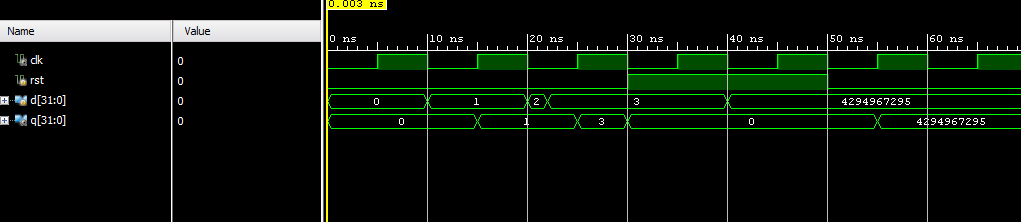
\includegraphics[width=0.9\textwidth]{H:/ELC-3338/MIPS_lab1/test_bench_image.png}
	\end{center}
\end{figure}



\section{Conclusions}
In this first lab, we set out to develop a program counter which would count sequentially within the span of a 32 bit register. This program counter was developed and tested under the expectations that it would be able to hold a starting value, count up from that value to an extent of 32 bits, and reset upon command. With the lab completed, we were able to meet these expectations testing the counter's ability to increment to the maximum capacity of 32 bits, as well as being able to reset the register to a desired value. In this lab, it was learned that it is not necessary to test every bit combination in the register to ensure functionality. In contrast, by ensuring that each bit is working, it is safe to believe that each combination can be achieved successfully.
\end{document} 